% --- LaTeX Homework Template - S. Venkatraman ---

% --- Set document class and font size ---

\documentclass[letterpaper, 11pt]{article}

% --- Package imports ---

\usepackage{
  amsmath, amsthm, amssymb, mathtools, dsfont,	  % Math typesetting
  graphicx, wrapfig, subfig, float,                  % Figures and graphics formatting
  listings, color, inconsolata, pythonhighlight,     % Code formatting
  fancyhdr, sectsty, hyperref, enumerate, enumitem, caption } % Headers/footers, section fonts, links, lists

% --- Page layout settings ---

% Set page margins
\usepackage[left=1.35in, right=1.35in, bottom=1in, top=1.1in, headsep=0.2in]{geometry}

% Anchor footnotes to the bottom of the page
\usepackage[bottom]{footmisc}
% Set line spacing
\renewcommand{\baselinestretch}{1.2}

% Set spacing between paragraphs
\setlength{\parskip}{1.5mm}

% Allow multi-line equations to break onto the next page
\allowdisplaybreaks

% Enumerated lists: make numbers flush left, with parentheses around them
\setlist[enumerate]{wide=0pt, leftmargin=21pt, labelwidth=0pt, align=left}
\setenumerate[1]{label={(\arabic*)}}

% --- Page formatting settings ---

% Set link colors for labeled items (blue) and citations (red)
\hypersetup{colorlinks=true, linkcolor=blue, citecolor=red}

% Make reference section title font smaller
\renewcommand{\refname}{\large\bf{References}}

% --- Settings for printing computer code ---

% Define colors for green text (comments), grey text (line numbers),
% and green frame around code
\definecolor{greenText}{rgb}{0.5, 0.7, 0.5}
\definecolor{greyText}{rgb}{0.5, 0.5, 0.5}
\definecolor{codeFrame}{rgb}{0.5, 0.7, 0.5}

% Define code settings
\lstdefinestyle{code} {
  frame=single, rulecolor=\color{codeFrame},            % Include a green frame around the code
  numbers=left,                                         % Include line numbers
  numbersep=8pt,                                        % Add space between line numbers and frame
  numberstyle=\tiny\color{greyText},                    % Line number font size (tiny) and color (grey)
  commentstyle=\color{greenText},                       % Put comments in green text
  basicstyle=\linespread{1.1}\ttfamily\footnotesize,    % Set code line spacing
  keywordstyle=\ttfamily\footnotesize,                  % No special formatting for keywords
  showstringspaces=false,                               % No marks for spaces
  xleftmargin=1.95em,                                   % Align code frame with main text
  framexleftmargin=1.6em,                               % Extend frame left margin to include line numbers
  breaklines=true,                                      % Wrap long lines of code
  postbreak=\mbox{\textcolor{greenText}{$\hookrightarrow$}\space} % Mark wrapped lines with an arrow
}

% Set all code listings to be styled with the above settings
\lstset{style=code}

% --- Math/Statistics commands ---

% Add a reference number to a single line of a multi-line equation
% Usage: "\numberthis\label{labelNameHere}" in an align or gather environment
\newcommand\numberthis{\addtocounter{equation}{1}\tag{\theequation}}

% Shortcut for bold text in math mode, e.g. $\b{X}$
\let\b\mathbf

% Shortcut for bold Greek letters, e.g. $\bg{\beta}$
\let\bg\boldsymbol

% Shortcut for calligraphic script, e.g. %\mc{M}$
\let\mc\mathcal

% \mathscr{(letter here)} is sometimes used to denote vector spaces
\usepackage[mathscr]{euscript}

% Convergence: right arrow with optional text on top
% E.g. $\converge[w]$ for weak convergence
\newcommand{\converge}[1][]{\xrightarrow{#1}}

% Normal distribution: arguments are the mean and variance
% E.g. $\normal{\mu}{\sigma}$
\newcommand{\normal}[2]{\mathcal{N}\left(#1,#2\right)}

% Uniform distribution: arguments are the left and right endpoints
% E.g. $\unif{0}{1}$
\newcommand{\unif}[2]{\text{Uniform}(#1,#2)}

% Independent and identically distributed random variables
% E.g. $ X_1,...,X_n \iid \normal{0}{1}$
\newcommand{\iid}{\stackrel{\smash{\text{iid}}}{\sim}}

% Equality: equals sign with optional text on top
% E.g. $X \equals[d] Y$ for equality in distribution
\newcommand{\equals}[1][]{\stackrel{\smash{#1}}{=}}

% Math mode symbols for common sets and spaces. Example usage: $\R$
\newcommand{\R}{\mathbb{R}}   % Real numbers
\newcommand{\C}{\mathbb{C}}   % Complex numbers
\newcommand{\Q}{\mathbb{Q}}   % Rational numbers
\newcommand{\Z}{\mathbb{Z}}   % Integers
\newcommand{\N}{\mathbb{N}}   % Natural numbers
\newcommand{\F}{\mathcal{F}}  % Calligraphic F for a sigma algebra
\newcommand{\El}{\mathcal{L}} % Calligraphic L, e.g. for L^p spaces

% Math mode symbols for probability
\newcommand{\pr}{\mathbb{P}}    % Probability measure
\newcommand{\E}{\mathbb{E}}     % Expectation, e.g. $\E(X)$
\newcommand{\var}{\text{Var}}   % Variance, e.g. $\var(X)$
\newcommand{\cov}{\text{Cov}}   % Covariance, e.g. $\cov(X,Y)$
\newcommand{\corr}{\text{Corr}} % Correlation, e.g. $\corr(X,Y)$
\newcommand{\B}{\mathcal{B}}    % Borel sigma-algebra

% Other miscellaneous symbols
\newcommand{\tth}{\text{th}}	% Non-italicized 'th', e.g. $n^\tth$
\newcommand{\Oh}{\mathcal{O}}	% Big-O notation, e.g. $\O(n)$
\newcommand{\1}{\mathds{1}}	% Indicator function, e.g. $\1_A$

% Additional commands for math mode
\DeclareMathOperator*{\argmax}{argmax}    % Argmax, e.g. $\argmax_{x\in[0,1]} f(x)$
\DeclareMathOperator*{\argmin}{argmin}    % Argmin, e.g. $\argmin_{x\in[0,1]} f(x)$
\DeclareMathOperator*{\spann}{Span}       % Span, e.g. $\spann\{X_1,...,X_n\}$
\DeclareMathOperator*{\bias}{Bias}        % Bias, e.g. $\bias(\hat\theta)$
\DeclareMathOperator*{\ran}{ran}          % Range of an operator, e.g. $\ran(T) 
\DeclareMathOperator*{\dv}{d\!}           % Non-italicized 'with respect to', e.g. $\int f(x) \dv x$
\DeclareMathOperator*{\diag}{diag}        % Diagonal of a matrix, e.g. $\diag(M)$
\DeclareMathOperator*{\trace}{trace}      % Trace of a matrix, e.g. $\trace(M)$

% Numbered theorem, lemma, etc. settings - e.g., a definition, lemma, and theorem appearing in that 
% order in Section 2 will be numbered Definition 2.1, Lemma 2.2, Theorem 2.3. 
% Example usage: \begin{theorem}[Name of theorem] Theorem statement \end{theorem}
\theoremstyle{definition}
\newtheorem{theorem}{Theorem}[section]
\newtheorem{proposition}[theorem]{Proposition}
\newtheorem{lemma}[theorem]{Lemma}
\newtheorem{corollary}[theorem]{Corollary}
\newtheorem{definition}[theorem]{Definition}
\newtheorem{example}[theorem]{Example}
\newtheorem{remark}[theorem]{Remark}

% Un-numbered theorem, lemma, etc. settings
% Example usage: \begin{lemma*}[Name of lemma] Lemma statement \end{lemma*}
\newtheorem*{theorem*}{Theorem}
\newtheorem*{proposition*}{Proposition}
\newtheorem*{lemma*}{Lemma}
\newtheorem*{corollary*}{Corollary}
\newtheorem*{definition*}{Definition}
\newtheorem*{example*}{Example}
\newtheorem*{remark*}{Remark}
\newtheorem*{claim}{Claim}

% --- Left/right header text (to appear on every page) ---

% Include a line underneath the header, no footer line
\pagestyle{fancy}
\renewcommand{\footrulewidth}{0pt}
\renewcommand{\headrulewidth}{0.4pt}

% Left header text: course name/assignment number
\lhead{CSE 5245 (Intro to Network Science) -- Lab 2}

% Right header text: your name
\rhead{Raman Ebrahimi}

% --- Document starts here ---

\begin{document}
\paragraph{Note:}I did this lab assignment by working with Kiante. Therefore, the results and the codes are similar.
\paragraph{Note:}The reason that I uploaded the results a bit late is that I was waiting for the code to compile one last time.
\subsection*{Code explanation}

\paragraph{}The first thing that was obstacle in this lab was the binary files. Binary files were not running on macOS, so we had to re-compile them to get their outputs. This was done by cloning GKlib, METIS, snap, and mlrmcl1.2 and compiling them using Terminal.

To get the outputs from the CNM algorithm for the YouTube dataset, I tried deleting nodes less than a threshold, which I tried deleting nodes with a degree less than 2 to 15, but the problem would remain, and the runtime was not changing much.

On the other hand, we could get the outputs for the other algorithms, and we changed the outputs' formats so we could use them for NetworkX pre-defined functions. These functions are in the Code Listing 1.

\begin{lstlisting}[language=python, caption={Functions for output formats}, label={lst:Pycode}]
def convert_communities_v2(G, communities):

    directed = False 
    dic = {}
    id_map = {} 
    node_num = 4039
    edge_num = 88234

    in_file = open(G, "rt")

    for line in in_file:
        if("#" in line):
            if("Nodes" in line):
                str_split = line.strip().split()
                node_num = int(str_split[2])
                edge_num = int(str_split[4])
                print(node_num, edge_num)
            continue
        str_split = [int(ele) for ele in line.strip().split()]
        if(str_split[0] == str_split[1]):
            continue
        if(str_split[0] in dic):
            dic[str_split[0]].append(str_split[1])
        else:
            dic[str_split[0]] = []
            dic[str_split[0]].append(str_split[1])
        if(directed == False):
            if(str_split[1] in dic):
                dic[str_split[1]].append(str_split[0])
            else:
                dic[str_split[1]] = []
                dic[str_split[1]].append(str_split[0])

    count = 1 
    key_set = [ele for ele in dic]
    for ele in key_set:
        id_map[ele] = count
        count += 1

    cres = []

    communityDict=defaultdict(set) # creates a dict of keys as community number and values as set of nodeIDs belonging to that community
    communityFile = open(communities, "rt") # the output file obtained from community detection algorithm is given in argv[2]

    outcount=1
    # finds the nodeID for the metics file by looping through the mapping dictionary of the metis file
    for ele in communityFile:
        for node, counts in id_map.items():
            if(outcount==counts):
                communityDict[ele].add(node)
        outcount+= 1

    for key, value in communityDict.items():
        cres.append(frozenset(value))

        return cres
\end{lstlisting}

Moreover, we used the following functions to get conductance and normalized cuts.
\begin{lstlisting}[language=python, caption={Functions for conductance and normalized cuts}, label={lst:Pycode}]

def conductance_scores(g, c, plot = True):
    c =  convert_communities(g,c)
    #how to get the conductance for all the communities
    conductance_scores_temp = [nx.conductance(g,communities_i, weight='weight') for communities_i in c]
    if plot == True:
        pd.Series(conductance_scores_temp).plot.hist(grid=True, bins=20, color='deepskyblue')
        plt.title('Conductance scores for each community')
        plt.xlabel('Conductance')
        plt.ylabel('Counts')
        plt.style.use('ggplot')
        plt.grid(axis='y', alpha=0.75)
        plt.show()
    return conductance_scores_temp
    
def ncs_scores(g, c, plot = False):
    c =  convert_communities(g,c)
    #how to get the conductance for all the communities
    ncs_scores_temp = [nx.normalized_cut_size(g,communities_i, weight='weight') for communities_i in c]
    if plot == True:
        pd.Series(ncs_scores_temp).plot.hist(grid=True, bins=20, color='deepskyblue')
        plt.title('Normalized cut scores for each community')
        plt.xlabel('Normalized cut')
        plt.ylabel('Counts')
        plt.style.use('ggplot')
        plt.grid(axis='y', alpha=0.75)
        plt.show()
    return ncs_scores_temp
\end{lstlisting}



\newpage
\subsection*{Results and comparisons}
\paragraph{}In figure~\ref{fig:youtube_prune} we plotted the degree distribution to decide on how to delete the nodes from youtube dataset. The best that out code gave us was the pruned youtube dataset with removing node with degrees less than 20. The runtime of this result was about 8 minutes.

\begin{figure}[h]
\centering
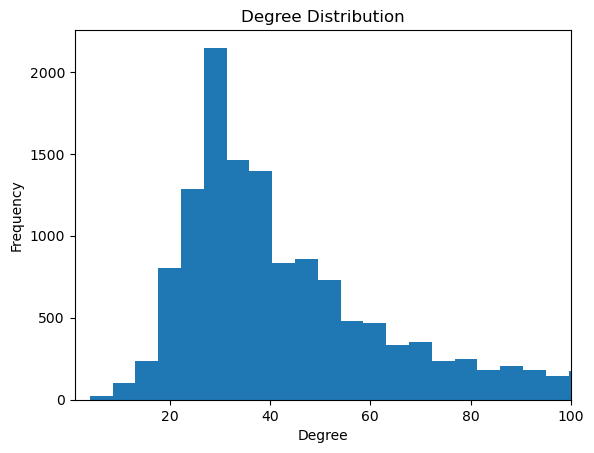
\includegraphics[width=0.5\textwidth]{output3.png}
\captionsetup{justification=centering,margin=0.5cm}
\caption{Degree distributions for youtube dataset for degrees between 0 and 100}
\label{fig:youtube_prune}
\end{figure}

As we can see in figure~\ref{fig:youtube_prune}, deleting the nodes with degrees than 20 seems good. The results have 40852 nodes and 834676 edges with a modularity score of 0.58 and 51 communities.

\paragraph{}After getting the desired format for the outputs, we used the networkx.algorithm.community library to compute the modularity of each output. In figure~\ref{fig:mod500}, we can see the bar plot for each dataset, except the YouTube dataset, and in figure~\ref{fig:clustering}, we can see two plots from the first lab assignment. 

\begin{figure}[h]
\centering
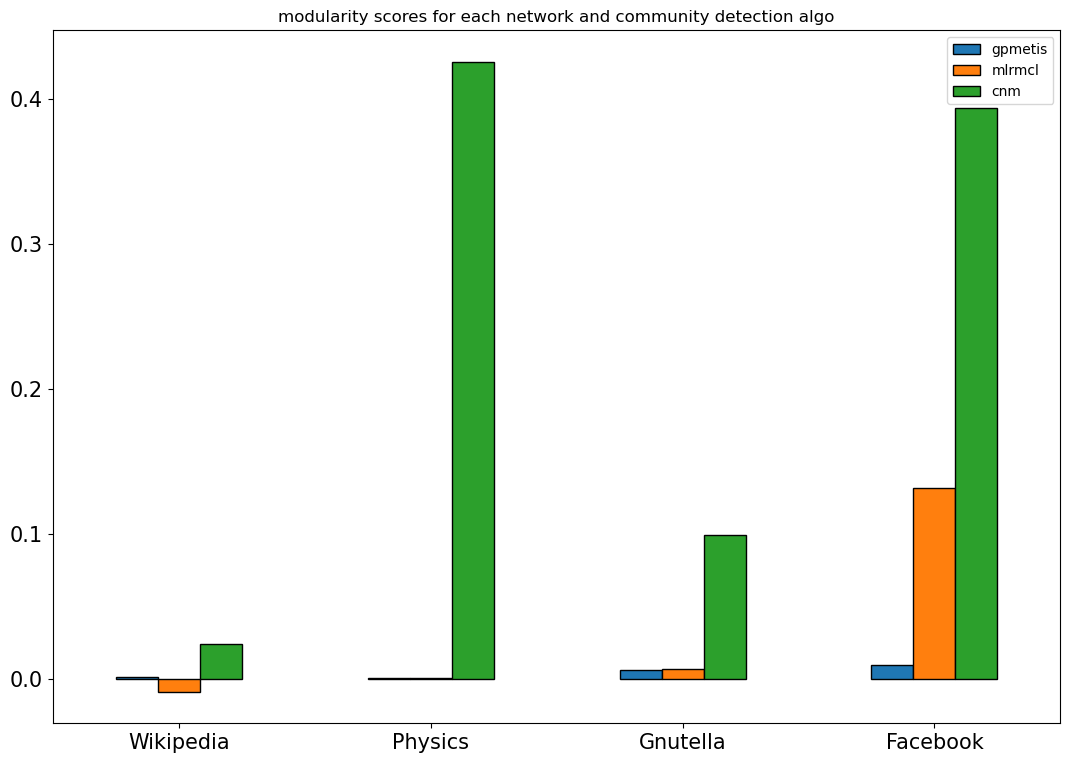
\includegraphics[width=0.5\textwidth]{output500.png}
\captionsetup{justification=centering,margin=0.5cm}
\caption{Modularity scores computed by different algorithms for each dataset.}
\label{fig:mod500}
\end{figure}

\begin{figure}[h]
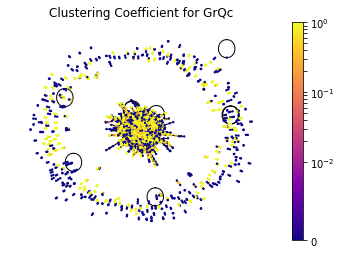
\includegraphics[width=0.5\textwidth]{GrQc_clustering.png}
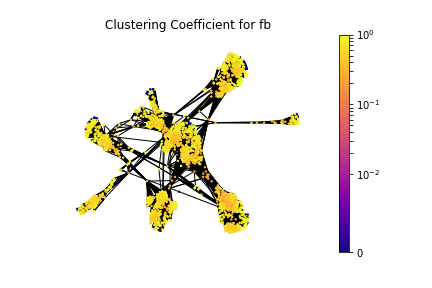
\includegraphics[width=0.5\textwidth]{fb_clustering.png}
\captionsetup{justification=centering,margin=0.5cm}
\caption{Heatmap for degree centrality and an approximate visualization of the network for Physics (left) and facebook (right).}
\label{fig:clustering}
\end{figure}

A high modularity score in a network means that the network can be divided into distinct modules or communities, with nodes within each module being more densely connected than nodes in other modules. In figure~\ref{fig:clustering}, we expect our algorithms to have high modularity scores in facebook and physics datasets. This is the case for the CNM algorithm, but we can't say they are successful for MLR-MCL and gpmetis.

Furthermore, by changing the -c 500 for MLR-MCL to -c 1000 and -c 10000 we got different results that are in figure~\ref{fig:c}.
\begin{figure}[h]
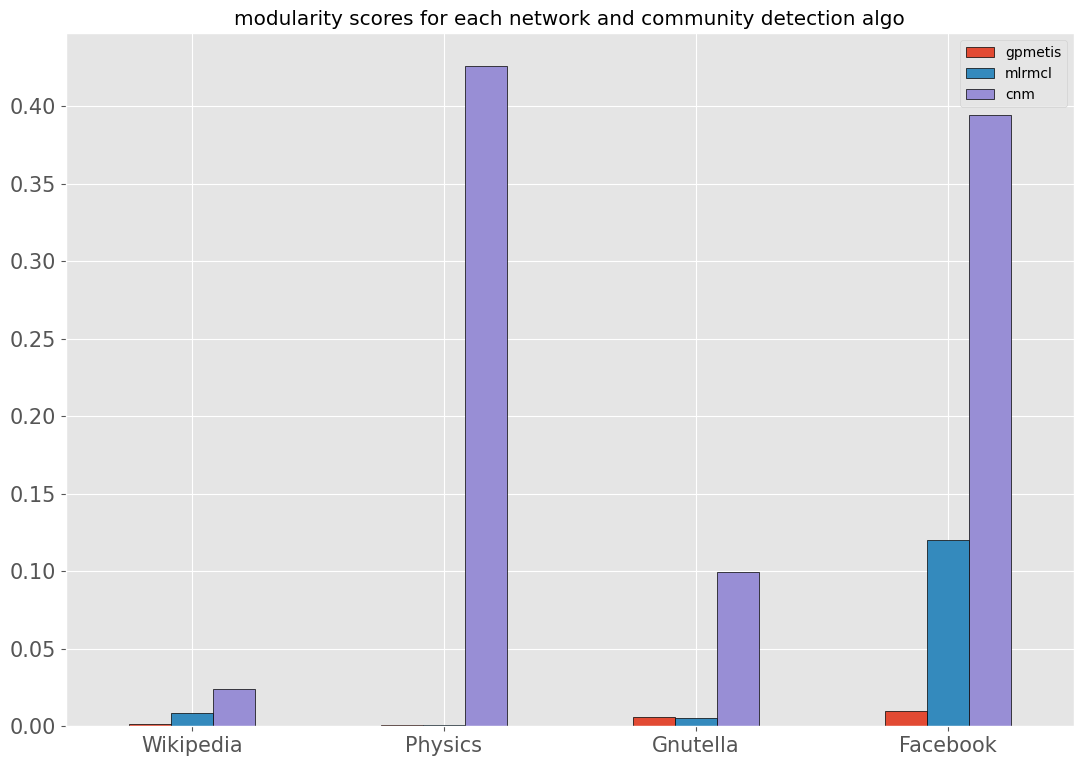
\includegraphics[width=0.5\textwidth]{output1000.png}
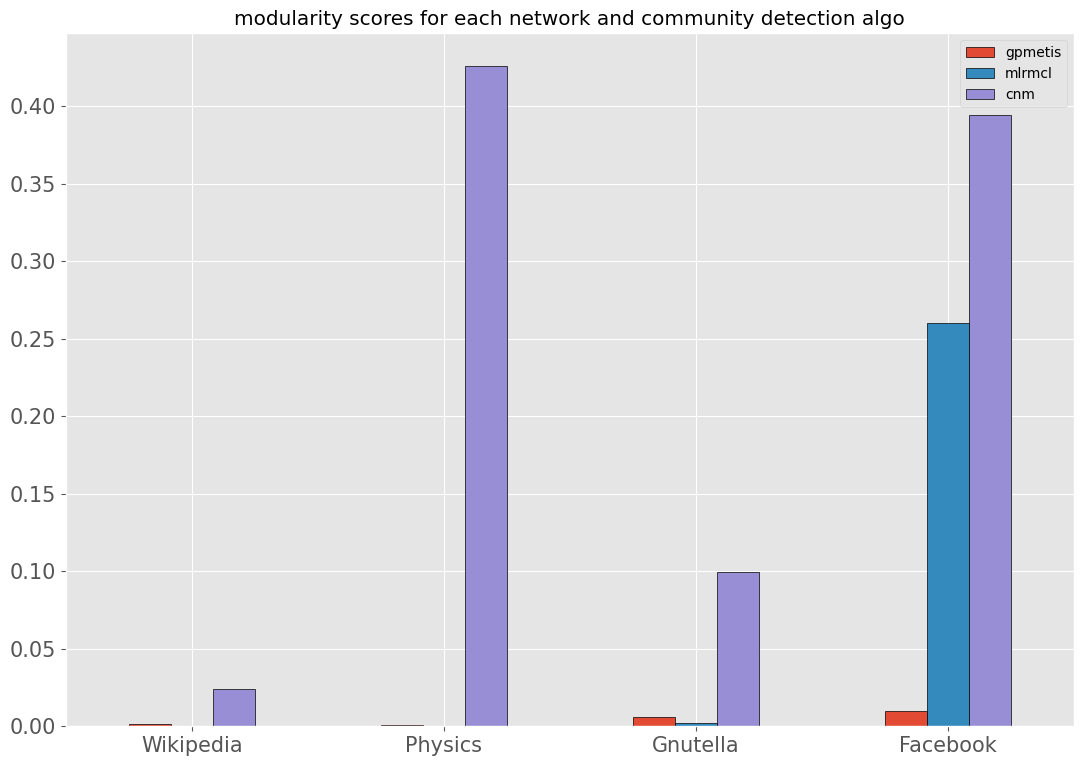
\includegraphics[width=0.5\textwidth]{output10000.png}
\captionsetup{justification=centering,margin=0.5cm}
\caption{Changing parameters on MLR-MCL to -c 1000 (left) and -c 10000 (right).}
\label{fig:c}
\end{figure}

As we can see, the score for facebook dataset grows but almost stays the same for other datasets.

\paragraph{Final note:}I waited for the final results but since the assignment is closed, I will send the files as they are and I will send the updated files after I have them.

\newpage

% --- Bibliography ---

% Start a bibliography with two items, a book and a webpage.
% To include a citation, use "\cite{book1}".

\begin{thebibliography}{2}

\bibitem{Networks, Crowds, and Markets: Reasoning about a Highly Connected World}
  Easley, David; Kleinberg Jon.
  \textit{Networks, Crowds, and Markets: Reasoning about a Highly Connected World}.
  Cambridge University Press, 2010.
  Print.
  
\bibitem{webpage1}
  ``Stanford Network Analysis Project''.
  SNAP, Stanford.
  Online. 
  \texttt{http://snap.stanford.edu/index.html}
  
\bibitem{webpage2}
  ``METIS''.
  Online. 
  \texttt{https://github.com/KarypisLab/METIS}


\bibitem{webpage3}
  ``GKlib''.
  Online. 
  \texttt{https://github.com/KarypisLab/GKlib}
  
  
\bibitem{webpage4}
  ``Network Analysis in Python''.
  NetworkX.
  Online. 
  \texttt{https://networkx.org/documentation/stable/reference/introduction.html}

\end{thebibliography}

% --- Document ends here ---

\end{document}